\documentclass[a4paper,11pt]{article}

\usepackage{amsmath}
\numberwithin{equation}{section}

\usepackage[qm]{qcircuit}
\usepackage{bibentry}




\usepackage{tikz,tikz-cd}



\usepackage{siunitx}
\usepackage{braket}
\usepackage{authblk}
\usepackage[a4paper, margin=1.5in]{geometry}
\usepackage{parskip}
\setlength{\parindent}{15pt}
\usepackage{tikz}
\usetikzlibrary{arrows, calc, patterns, angles, quotes}
\usetikzlibrary{decorations.pathmorphing}
\usepackage{amssymb}
\usetikzlibrary{shapes.geometric}
\usepackage[section]{placeins}
\usepackage{pgfplots}
\usepackage{clock}
\usepackage[clock]{ifsym}
\usetikzlibrary{shapes}
\usepackage{amsthm}
\theoremstyle{definition}
\usepackage{empheq}
\usepackage{hyperref}
\usepackage{tensor}
\usepackage{xcolor}
\hypersetup{
	colorlinks,
	linkcolor={black!50!black},
	citecolor={blue!50!black},
	urlcolor={blue!80!black}
}
\newcommand{\p}{\partial}
\newcommand{\lag}{\mathcal{L}}
\newcommand{\E}{\mathcal{E}}

\newcommand{\nn}{\nonumber}

\newcommand{\M}{\mathcal{M}}
\newcommand{\V}{\mathbf{V}}
\newcommand{\W}{\mathbf{W}}
\newcommand{\X}{\mathbf{X}}
\newcommand{\A}{\mathcal{A}}

\newcommand{\f}[2]{\frac{#1}{#2}}

\newcommand{\ift}{\infty}

\newcommand{\lp}{\left(}
\newcommand{\rp}{\right)}

\newcommand{\lb}{\left[}
\newcommand{\rb}{\right]}

\newcommand{\lc}{\left\{}
\newcommand{\rc}{\right\}}
%\usepgfplotslibrary{external}
%\tikzexternalize

\begin{document}
\begin{titlepage}\centering
 \clearpage
 \title{\textsc{\bf{Matrices in Quantum Computing}}\\\smallskip A 2-qubit Entangler Circuit\\}
 \author{\bigskip Huan Q. Bui}
 \affil{Colby College CLAS 2019\\$\,$\\ PHYSICS \& MATHEMATICS\\ Statistics \\$\,$\\Class of 2021\\}
 \date{\today}
 \maketitle
 \thispagestyle{empty}
\end{titlepage}

\newpage

\tableofcontents

\newpage

\section{Introduction}

Quantum computing and quantum information science are rapidly growing fields in recent years. Progress is made everyday in not only in the physics labs but also in the mathematical foundation, most of which is linear algebra. The matrix theory behind quantum computing is voluminous, and thus it would be insane for me to talk about all kinds of matrices in quantum computing. So today, I would like to draw your attention to one of the simplest and basic yet interesting circuits in all of quantum computing: the 2-qubit entanglement circuit, and some of the matrix theory behind it. 

\begin{center}
	$\,$\Qcircuit @C=.7em @R=.4em  {
		\lstick{a: \ket{0}} & \qw & \qw & \targ & \meter & \qw \\
		\lstick{b: \ket{0}} & \qw & \gate{H} & \ctrl{-1}& \meter & \qw 
	}
\end{center}

\section{Presentation layout}
Here's my plan for this presentation. I will 
\begin{enumerate}
	\item first provide some background on quantum computing. I will introduce some of the basic objects in quantum computing such as qubits, quantum circuits, quantum gates, and entanglement. 
	\item And as I introduce these objects, the mathematical concepts of the Kronecker product and tensor product will come up, as they are the building blocks of the theory of quantum computation. I will talk about what these matrix theories are, how they work, and, time permitting, ``why'' they are required.
	\item  Then, we will walkthrough the 2-qubit entanglement circuit that I have just shown. We will see how the tensor product appears and how we can use it ``see'' what the circuit actually does.
	\item Finally, I will show how you can actually implement this circuit (or any other circuit) on your browser and have an actual quantum computer at IBM execute the commands.
\end{enumerate}

\section{Qubits}
So let us start with qubits. Qubits are kind of like classical bits, but not really. Classical bits can take values of only 0 and 1, ``on'' or ``off'', ``up'' or ``down,'' while quantum bits can take any ``superposition'' of those two states, since qubits are quantum mechanical objects.

\begin{figure}[h!]
	\centering
	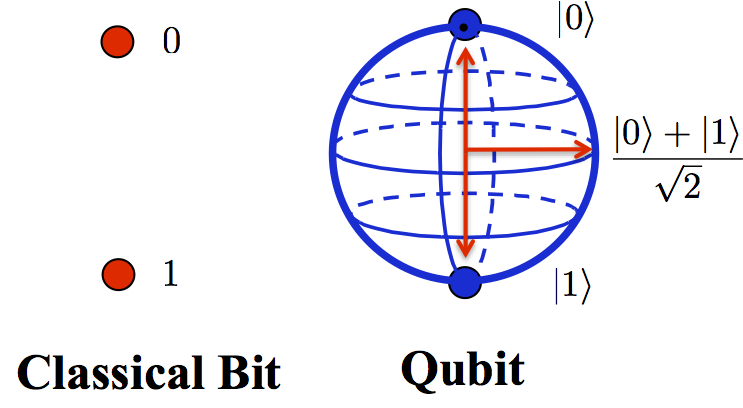
\includegraphics[scale=0.5]{atom1.png}
\end{figure}

Most of the time, qubits are individual atoms that can be excited to the excited state or de-excited into the ground state. Mathematically, we can think of these states as forming a basis for the space of all possible states of the atom, and the state of a qubit can be represented by the following linear combination:
\begin{align*}
a\begin{bmatrix}
1\\0
\end{bmatrix}
+
b\begin{bmatrix}
0\\1
\end{bmatrix},
\end{align*} 
where 
$
\begin{bmatrix}
1\\0
\end{bmatrix} \text{represents the ground state, and}
\begin{bmatrix}
0\\1
\end{bmatrix} \text{represents the excited state}
$. The coefficients $a,b$ are complex numbers such that the sum of the modulus squares is one:
\begin{align*}
\vert a \vert^2 + \vert b\vert^2 = 1,
\end{align*}
the reason being, in quantum mechanics, it is require that the magnitude of the state vector is 1. In fact, in physics, it is often interpreted that $\vert a \vert^2$ is the probability of the qubit being in the ground state, and $\vert b\vert$ is the probability of the qubit being in the excited state. 

Now, before we move on, for the sake of convenience, let us introduce a new notation for the basis states of a qubit. Let $\ket{0}$ represent the vector $\begin{bmatrix}
1 & 0
\end{bmatrix}^\top$ and $\ket{1}$ represent the vector $\begin{bmatrix}
0&1
\end{bmatrix}^\top$. The reason for doing this is that now we can just call the ground state the ``zero'' state and excited state the ``one'' state, giving us a nice way to relate the basis values of a classical bit. So, the state of single qubit can be  written as
\begin{align*}
a\ket{0} + b\ket{1}.
\end{align*}



\section{Quantum gates}
Another fundamental object in quantum computing is quantum gates. If we think of states of qubits as vectors, then quantum gates are modeled by linear transformations - matrices - on the state vectors of qubits. For example, one of the most common and important single-qubit quantum gates, is called the Hadamard gate, which is in matrix form is
\begin{align*}
H = \f{1}{\sqrt{2}}\begin{bmatrix}
1&1\\
1&-1
\end{bmatrix}.
\end{align*}
This gate is actually the first component on the quantum circuit we have seen:
\begin{center}
	$\,$\Qcircuit @C=.7em @R=.4em  {
		\lstick{a: \ket{0}} & \qw & \qw & \targ & \meter & \qw \\
		\lstick{b: \ket{0}} & \qw & \gate{H} & \ctrl{-1}& \meter & \qw 
	}
\end{center}
The Hadamard gate is denoted with an $H$. We can see what $H$ does to, say $\ket{0}$:
\begin{align*}
H\ket{0} = H\begin{bmatrix}
1\\0
\end{bmatrix} = \f{1}{\sqrt{2}}\begin{bmatrix}
1&1\\1&-1
\end{bmatrix}\begin{bmatrix}
1\\0
\end{bmatrix} = \f{1}{\sqrt{2}}\begin{bmatrix}
1\\1
\end{bmatrix},
\end{align*}
which we can equivalently write as
\begin{align*}
\f{1}{\sqrt{2}}\ket{0} + \f{1}{2}\ket{1}.
\end{align*}
So what the Hadamard gate does is putting a pure state into a perfect superposition, with exactly 50\% chance of finding the qubit either state $\ket{0}$ or $\ket{1}$. 


\section{Multiple qubits}
Like classical circuits, quantum circuits require multiple qubits to operate. And so a natural question to ask now is how do we represent the quantum state of 2-qubits with the same vector. Let us say that the qubit 1 has state $$a\ket{0} + b\ket{1} = \begin{bmatrix}
a\\b
\end{bmatrix}$$ and qubit 2 has state $$c\ket{0} + d\ket{1} = \begin{bmatrix}
c\\d
\end{bmatrix}.$$ It is clear that we can neither add, nor ``multiply'' these ``pairs'' in any traditional way in order to get a vector of unit length. It turns out that we can represent the state of two qubits by do the following seemingly ``magical'' multiplication procedure,
\begin{align*}
\begin{bmatrix}
a\\b
\end{bmatrix}
\boxtimes
\begin{bmatrix}
c\\d
\end{bmatrix} = \begin{bmatrix}
a\begin{bmatrix}
c\\d
\end{bmatrix}\\
b\begin{bmatrix}
c\\d
\end{bmatrix}
\end{bmatrix}
=
\begin{bmatrix}
ac\\ad\\bc\\bd
\end{bmatrix}.
\end{align*}
We can check quite easily that this new vector has unit length. Applying this procedure to the basis states $\ket{0}$, $\ket{1}$, we actually get a basis for the vector space that contains all possible quantum states of two qubits:
\begin{align*}
\ket{0}\boxtimes \ket{0}
=
\begin{bmatrix}
1\\0\\0\\0
\end{bmatrix}, \ket{0}\boxtimes \ket{1}
=
\begin{bmatrix}
0\\1\\0\\0
\end{bmatrix}, \ket{1}\boxtimes \ket{0}
=
\begin{bmatrix}
0\\0\\1\\0
\end{bmatrix}, \ket{1}\boxtimes \ket{1}
=
\begin{bmatrix}
0\\0\\0\\1
\end{bmatrix}, 
\end{align*}
and so it is convenient for us to write
\begin{align*}
\ket{00} = \ket{0} \boxtimes \ket{0}\\
\ket{01} = \ket{0} \boxtimes \ket{1}\\
\ket{10} = \ket{1} \boxtimes \ket{0}\\
\ket{11} = \ket{1} \boxtimes \ket{1}
\end{align*}
where the first slot indicates the (pure) state of the first qubit, and the second slot indicates the (pure) state of the second qubit. And so it is not so hard to see that
\begin{align*}
\begin{bmatrix}
a\\b
\end{bmatrix}
\boxtimes
\begin{bmatrix}
c\\d
\end{bmatrix} = ac\ket{00} + ad\ket{01} + bc\ket{10} + bd\ket{11}. 
\end{align*}

\section{Elementariness \& Entanglement}
With this, we can see that given two qubits with defined states, this ``product'' always gives us a new two-qubit joint state, and we call this joint state \textbf{elementary}. Now, we might wonder whether any joint state can be expressed as this special product of two single-qubit states. It turns out that the answer is no. 

This is a subtle fact. So, let us consider an analogue to this, with polynomials. Let us consider $p(x)$ a polynomial in $x$ and $q(y)$ a polynomial in $y$. It is clear that $p(x)\cdot q(y)$ is a polynomial of both $x$ and $y$. However, this polynomial with both $x$ and $y$,
\begin{align*}
xy + 1,
\end{align*}
cannot be written as a product of a polynomial in $x$ and one in $y$. 

Back to qubits. Consider the following example. This joint state
\begin{align*}
\frac{1}{\sqrt{2}}\begin{bmatrix}
1\\0\\0\\1
\end{bmatrix} = \f{1}{\sqrt{2}}\ket{00} + \f{1}{\sqrt{2}}\ket{11}
\end{align*}
while can written as a linear combination of products of basis states, cannot be written as a single product of two single-qubit states. These qubits are now in a state we call \textbf{entanglement}. 

Why this terminology? If we stare at the state vector above for a bit, we can see that the two-qubit is either in the state $\ker{00}$ or $\ket{11}$ with equal probability. So we can make a measurement on the first qubit, for example, and see $\ket{0}$, then we immediately know with high very high confidence that the state of the second qubit is $\ket{0}$ without measuring it. And because this feels very much like the two qubits are somehow ``coordinating'' they are said to be ``entangled.''

\section{Kronecker product}

Now that we are able to represent a system of qubits with a single vector. What about matrices that act on these vectors? It turns out that if $\mathcal{A}$ is some matrix that acts on the first qubit, and $\mathcal{B}$ is some matrix that acts on the second qubit, then the corresponding matrix that acts on the two-qubit state is given by
\begin{align*}
\A\ket{a} \boxtimes \mathcal{B}\ket{b} = (\A \otimes \mathcal{B})(\ket{a} \boxtimes \ket{b})
\end{align*}
where ``$\otimes$'' is called the \textbf{Kronecker product}. And the way the Kronecker product is defined is kind of similar to how the magical product ``$\boxtimes$'' was defined before. The Kronecker product of two matrices is defined as follows. If we are given two matrices
\begin{align*}
\A = \begin{bmatrix}
m & n \\ o & p
\end{bmatrix}
\hspace{0.5cm}
\mathcal{B} = \begin{bmatrix}
q & r & s \\ t & u & v \\ w&x&y
\end{bmatrix}
\end{align*} 
then the Kronecker product of $\mathcal{A}$ and $\mathcal{B}$ is a $6\times 6$ matrix:
\begin{align*}
\A \otimes \mathcal{B} = \begin{bmatrix}
m\begin{bmatrix}
q & r & s \\ t & u & v \\ w&x&y
\end{bmatrix} & n\begin{bmatrix}
q & r & s \\ t & u & v \\ w&x&y
\end{bmatrix}\\
o\begin{bmatrix}
q & r & s \\ t & u & v \\ w&x&y
\end{bmatrix} & p\begin{bmatrix}
q & r & s \\ t & u & v \\ w&x&y
\end{bmatrix}
\end{bmatrix}
=
\begin{bmatrix}
mq & mr & ms & nq & nr & ns\\
mt & mu & mv & nt & nu & nv\\
mw & mx & ms & nw & nx & ny\\
oq & or & os & pq & pr & ps\\
ot & ou & ov & pt & pu & pv\\
ow & ox & oy & pw & px & pys\\
\end{bmatrix}
\end{align*}

We can look back at our circuit diagram:
\begin{center}
	$\,$\Qcircuit @C=.7em @R=.4em  {
		\lstick{a: \ket{0}} & \qw & \qw & \targ & \meter & \qw \\
		\lstick{b: \ket{0}} & \qw & \gate{H} & \ctrl{-1}& \meter & \qw 
	}
\end{center}
and check that this definition of the Kronecker product makes sense, i.e., the left hand side where we have single-qubit gates acting on individual qubits:
\begin{align*}
I\ket{0} \boxtimes H\ket{1} &= \begin{bmatrix}
1 & 0 \\  0 & 1
\end{bmatrix}\begin{bmatrix}
1 \\ 0
\end{bmatrix} \boxtimes \f{1}{\sqrt{2}}\begin{bmatrix}
1 & 1\\ 1 & -1
\end{bmatrix}\begin{bmatrix}
0 \\ 1
\end{bmatrix}\\
&= \begin{bmatrix}
1 \\ 0
\end{bmatrix} \boxtimes \f{1}{\sqrt{2}}\begin{bmatrix}
1 \\ 1
\end{bmatrix} \\
&= \f{1}{\sqrt{2}}\begin{bmatrix}
1\\1\\0\\0
\end{bmatrix}
\end{align*}
is equal to the right hand side, where we have a two-qubit gate acting on a two-qubit state vector:
\begin{align*}
(I \otimes H)(\ket{0} \boxtimes \ket{0}) = \begin{bmatrix}
\f{1}{\sqrt{2}}\begin{bmatrix}
1&1\\1&-1
\end{bmatrix} & \mathcal{O}\\
\mathcal{O} & \f{1}{\sqrt{2}}\begin{bmatrix}
1&1\\1&-1
\end{bmatrix} 
\end{bmatrix}\begin{bmatrix}
1\\0\\0\\0
\end{bmatrix} = \f{1}{\sqrt{2}}\begin{bmatrix}
1\\1\\0\\0
\end{bmatrix}.
\end{align*}



\section{Some properties \& Elementariness}
So it appears that the $\otimes$ product is very similar to the $\boxtimes$ product. In fact, we can notice a few things:
\begin{enumerate}
	\item Both are \textbf{bilinear}, i.e., linear in both the first and second argument. 
	\item Both are \textbf{distributive}, left and right. We in fact have seen these properties before when we wrote
	\begin{align*}
	\begin{bmatrix}
	a\\b
	\end{bmatrix}
	\boxtimes
	\begin{bmatrix}
	c\\d
	\end{bmatrix} = ac\ket{00} + ad\ket{01} + bc\ket{10} + bd\ket{11}. 
	\end{align*}
	By tweaking the left hand side, the bilinear and distributive properties become very clear:
	\begin{align*}
	(a\ket{0} + b\ket{1})\boxtimes (c\ket{0} + d\ket{1}) = ac\ket{00} + ad\ket{01} + bc\ket{10} + bd\ket{11}. 
	\end{align*}
	\item Both are \textbf{associative}, which can easily be checked.
	\item Both are \textbf{NOT commutative}. For example, $\ket{01} \neq \ket{10}$.
	\item It also turns out that the business with elementariness also carries over into Kronecker products of matrices. What I mean is that, say, given two $2\times 2$ matrices, their Kronecker product is a $4\times 4$ matrix (which is what we just did). But not every $4\times 4$ matrix can be written as a Kronecker product of two $2\times 2$ matrices. An example can be readily found in our quantum circuit:
	\begin{center}
		$\,$\Qcircuit @C=.7em @R=.4em  {
			\lstick{a: \ket{0}} & \qw & \qw & \targ & \meter & \qw \\
			\lstick{b: \ket{0}} & \qw & \gate{H} & \ctrl{-1}& \meter & \qw 
		}
	\end{center}

	The last gate before the measurements is called the $Control-NOT$ gate. It is a conditional bit-flip gate, conditioned on the second qubit. In matrix form,
	\begin{align*}
	CNOT_b = \begin{bmatrix}
	1 & 0 & 0 & 0\\
	0 & 0 & 0 & 1\\
	0 & 0 & 1 & 0\\
	0 & 1 & 0 & 0
	\end{bmatrix} \hspace{0.5cm} \longrightarrow \begin{cases}
	\ket{00} \to \ket{00}\\
	\ket{10} \to \ket{10}\\
	\ket{01} \to \ket{11}\\
	\ket{11} \to \ket{01}
	\end{cases}
	\end{align*}
	Quantum gates that are not elementary are also called ``entangled.''

\end{enumerate}




\section{Entanglement circuit}

So, we look back at the quantum circuit
\begin{center}
	$\,$\Qcircuit @C=.7em @R=.4em  {
		\lstick{a: \ket{0}} & \qw & \qw & \targ & \meter & \qw \\
		\lstick{b: \ket{0}} & \qw & \gate{H} & \ctrl{-1}& \meter & \qw 
	}
\end{center}
we realize that we have seen how every component works. We don't have to worry so much about what the measurement gates. Technically speaking, they are not exactly quantum gates, since what they do is projecting the state vector onto one of the basis states $\ket{0}$ or $\ket{1}$. Nevertheless, since we already know how each quantum gate in this circuit functions, we can sort of work through the circuit and see why this circuit does what it does - entangling two qubits.
\begin{enumerate}
	\item First, the identity gate doesn't do anything to the first qubit. But the second qubit is subjected to the Hadamard which puts it in a perfect superposition. So we have
	\begin{align*}
	&a : \ket{0} \to \ket{0}\\
	&b : \ket{0} \to \f{1}{\sqrt{2}}\ket{0}+ \f{1}{\sqrt{2}}\ket{1}. 
	\end{align*} 
	\item Then, the $CNOT$ gate acts on the two-qubit state:
	\begin{align*}
	CNOT_b \lb\ket{0} \boxtimes \lp \f{1}{\sqrt{2}} \ket{0} + \f{1}{\sqrt{2}} \ket{1} \rp\rb
	= 
	\begin{bmatrix}
	1 & 0 & 0 & 0\\
	0 & 0 & 0 & 1\\
	0 & 0 & 1 & 0\\
	0 & 1 & 0 & 0
	\end{bmatrix}
	\begin{bmatrix}
	1/\sqrt{2} \\ 1/\sqrt{2} \\ 0\\0
	\end{bmatrix} 
	= 
	\f{1}{\sqrt{2}} \begin{bmatrix}
	1\\0\\0\\1
	\end{bmatrix},
	\end{align*}
	which is exactly what we have said before:
	\begin{align*}
	\f{1}{\sqrt{2}} \begin{bmatrix}
	1\\0\\0\\1
	\end{bmatrix} 
	= \f{1}{\sqrt{2}}\ket{00} + \f{1}{\sqrt{2}}\ket{11},
	\end{align*}
	and entangled state.  
	
	
\end{enumerate}

\section{Simulation on IBM-Q}

There's a website by IBM called the IBM-Q experience that lets us upload/design a quantum circuit and have an actual quantum computer at IBM execute the circuit. Here is what I got when I ran this circuit:
	\begin{figure}[h!]
	\centering
	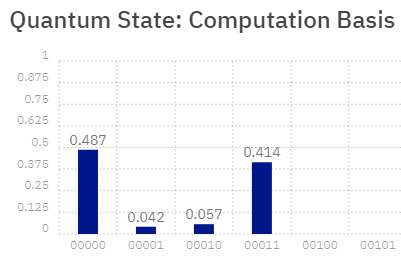
\includegraphics[scale=0.8]{ibmq1.png}
\end{figure}
As you can see, the probabilities of measuring $\ket{00}$ and $\ket{11}$ are roughly equal. One thing to notice is that there are errors, which is due to the quantum mechanical - probabilistic nature of the computation. 




\section{Tensor Products}

Finally, there is one more piece to my talk, that is the connection between the ``magical product'' denoted as $\boxtimes$ and the Kronecker product, $\otimes$. As you might have guessed, or had an intuitive feel for, the $\boxtimes$ and $\otimes$ are very much the same - because they are! In fact, they are instances, or representations, of what's called the \textbf{tensor product}. So, the notation $\boxtimes$ is just my way of not confusing myself and you guys. In reality, the tensor product is denoted by $\otimes$. 

So why exactly do we use the tensor product to describe the state of multiple qubits and what exactly is the tensor product? The answer to the first question is not so satisfying: because the tensor product is one that works, and that it is postulated in quantum mechanics that the joint state of two quantum states \textit{is} the tensor product of the two individual quantum states. 

The answer to the second question is a little more subtle and interesting. Like I said, the Kronecker product and $\boxtimes$ are instances of the tensor product. Kronecker products are special kind of product on matrices, same for $\boxtimes$, since we can always think about a vector as a very tall and very narrow matrix. On the other hand, the tensor product is one of vector spaces and of linear functions on vector spaces in general.

\begin{center}
\begin{tikzcd}[row sep=15ex, column sep=20ex]
	\V \otimes \W  \arrow[r, "linear"', "\hat{f}"]  & \X
	\\ \V \times \W \arrow[ur, "f", "bilinear"'] \arrow[u, hook, "\phi"]
\end{tikzcd}
\end{center}

Roughly speaking, the tensor product of two vector spaces is a new vector space. But the tensor product is constructed in such a way that if somebody gives me a bilinear function from the Cartesian product space to some target space, then I immediately have a \textbf{unique} corresponding linear function from the tensor product space to the same target space. 

Since we are working with operators, we can consider the case where $\X$ is $\V \otimes \W$ itself. Let's say we given an operator $\lag$ on $\V$ and $\M$ on $\W$.

\begin{center}
	\begin{tikzcd}[row sep=15ex, column sep=20ex]
		\V \otimes \W  \arrow[r, "linear"', "\hat{f}"]  & \V\otimes \W
		\\ \V \times \W \arrow[ur, "f", "bilinear"'] \arrow[u, hook, "\phi"]
	\end{tikzcd}
\end{center} 

We know that $\lag \otimes \M$ is an operator on $\V\otimes \W$, and that $\lag[v]\otimes \M[w]$ is a bilinear function from $\V\times \W$ to $\V\otimes \W$. And so by the uniqueness in the definition, it must be true that
\begin{align*}
(\lag\otimes \M)(v\otimes w) = \lag[v]\otimes \M[w].
\end{align*} 
This looks every much like how the Kronecker product is defined, as except here $\lag$, $\M$ are general linear functions, not matrices. And while there is not a general definition for how to compute the tensor product of two linear functions, we don't have to worry so much because if possible, we can always choose a basis $\nu$ for $\V$ and $\omega$ for $\W$ with respect to which $\lag$ and $\M$ can be represented by matrices. And so the matrix of $\lag\otimes \M$ with respect to a basis $\tau$ of $\V\otimes \W$ created by tensor products of the elements of $\nu, \omega$ can be calculated via the Kronecker product. 
\begin{align*}
[\lag\otimes \M]_{\tau\leftarrow \tau} = [\lag]_{\nu\leftarrow\nu} \otimes [\M]_{\omega\leftarrow\omega}.
\end{align*}
And so we're done.

\section{Recap}
And so, just to summarize, in this talk we have learned a few things from trying to figure out how a 2-qubit entanglement circuit works. We have seen what qubits and quantum gates are, and how the Kronecker product and matrix representations of these objects allow us to model a quantum computation and calculate numerical results. We also learn about entanglement and how entanglement manifests in the language of matrix theory. Finally, we look at a more general concept of the Kronecker product on matrices, called the tensor product. 


\section{Why quantum computers?}

At this point, it would be natural to question the fidelity of quantum computations. Are answers reliable? And why quantum computation? How is quantum computation ``better'' than classical computation with bits and deterministic processes? The main advantage of quantum computation is resources. Because one qubit can store much more information than a single classical bit can due to its quantum mechanical-probabilistic nature, quantum computers can do certain things much faster and more efficiently than classical computers can such as factoring numbers or optimization problems or where quantum parallelism proves superior. 


\end{document}